\question[10]
\mbox{}
\begin{center}
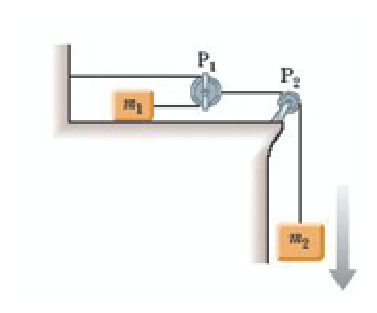
\includegraphics [scale=0.7]{latex/eps/1_5_1_image_1.eps}
%\caption{Gambar katrol}
\end{center}
Sebuah objek bermassa $m_{1}$ berada pada meja horizontal. $m_{1}$ dihubungkan dengan $m_{2}$ oleh katrol tak bermassa $P_{1}$ dan $P_{2}$ seperti pada gambar.\\
a$)$ Cari hubungan percepatan benda 2 dengan percepatan benda 1 ? \\
b$)$ Cari tegangan tali ?\\
c$)$ Cari percepatan benda 1 dan benda 2 dalam $m_{1}$, $m_{2}$, dan $g$ ?
